%!TEX ROOT=../emnlp2023.tex

\section{Introduction}
\label{sec:introduction}
We release a pipeline for fact-checking claims using evidence retrieved from the web consisting of two modules -- a \textit{retriever}, which picks the most relevant sources among the available knowledge store\footnote{Due to the pre-retrieval step that was used to generate knowledge stores, our \say{retriever} module could more conventionally be referred to as a \say{reranker}, which we refrain from, to avoid confusion with reranking steps it uses as a subroutine.} and an \textit{evidence \& label generator} which generates evidence for the claim using these sources, as well as its veracity label. 

Our pipeline is a variant of the popular Retrieval-augmented Generation (RAG) scheme~\cite{rag}, making it easy to re-implement using established frameworks such as Langchain, Haystack, or our attached Python codebase for future research or to use as a baseline.

This paper describes our pipeline and the decisions taken at each module, achieving a simple yet efficient RAG scheme that improves dramatically across the board over the baseline system from~\cite{averitec2024}, and scores third in the \averitec{}  leaderboard as of August 2024.

% show figures/pipeline.png
\begin{figure}[h]
    \centering
    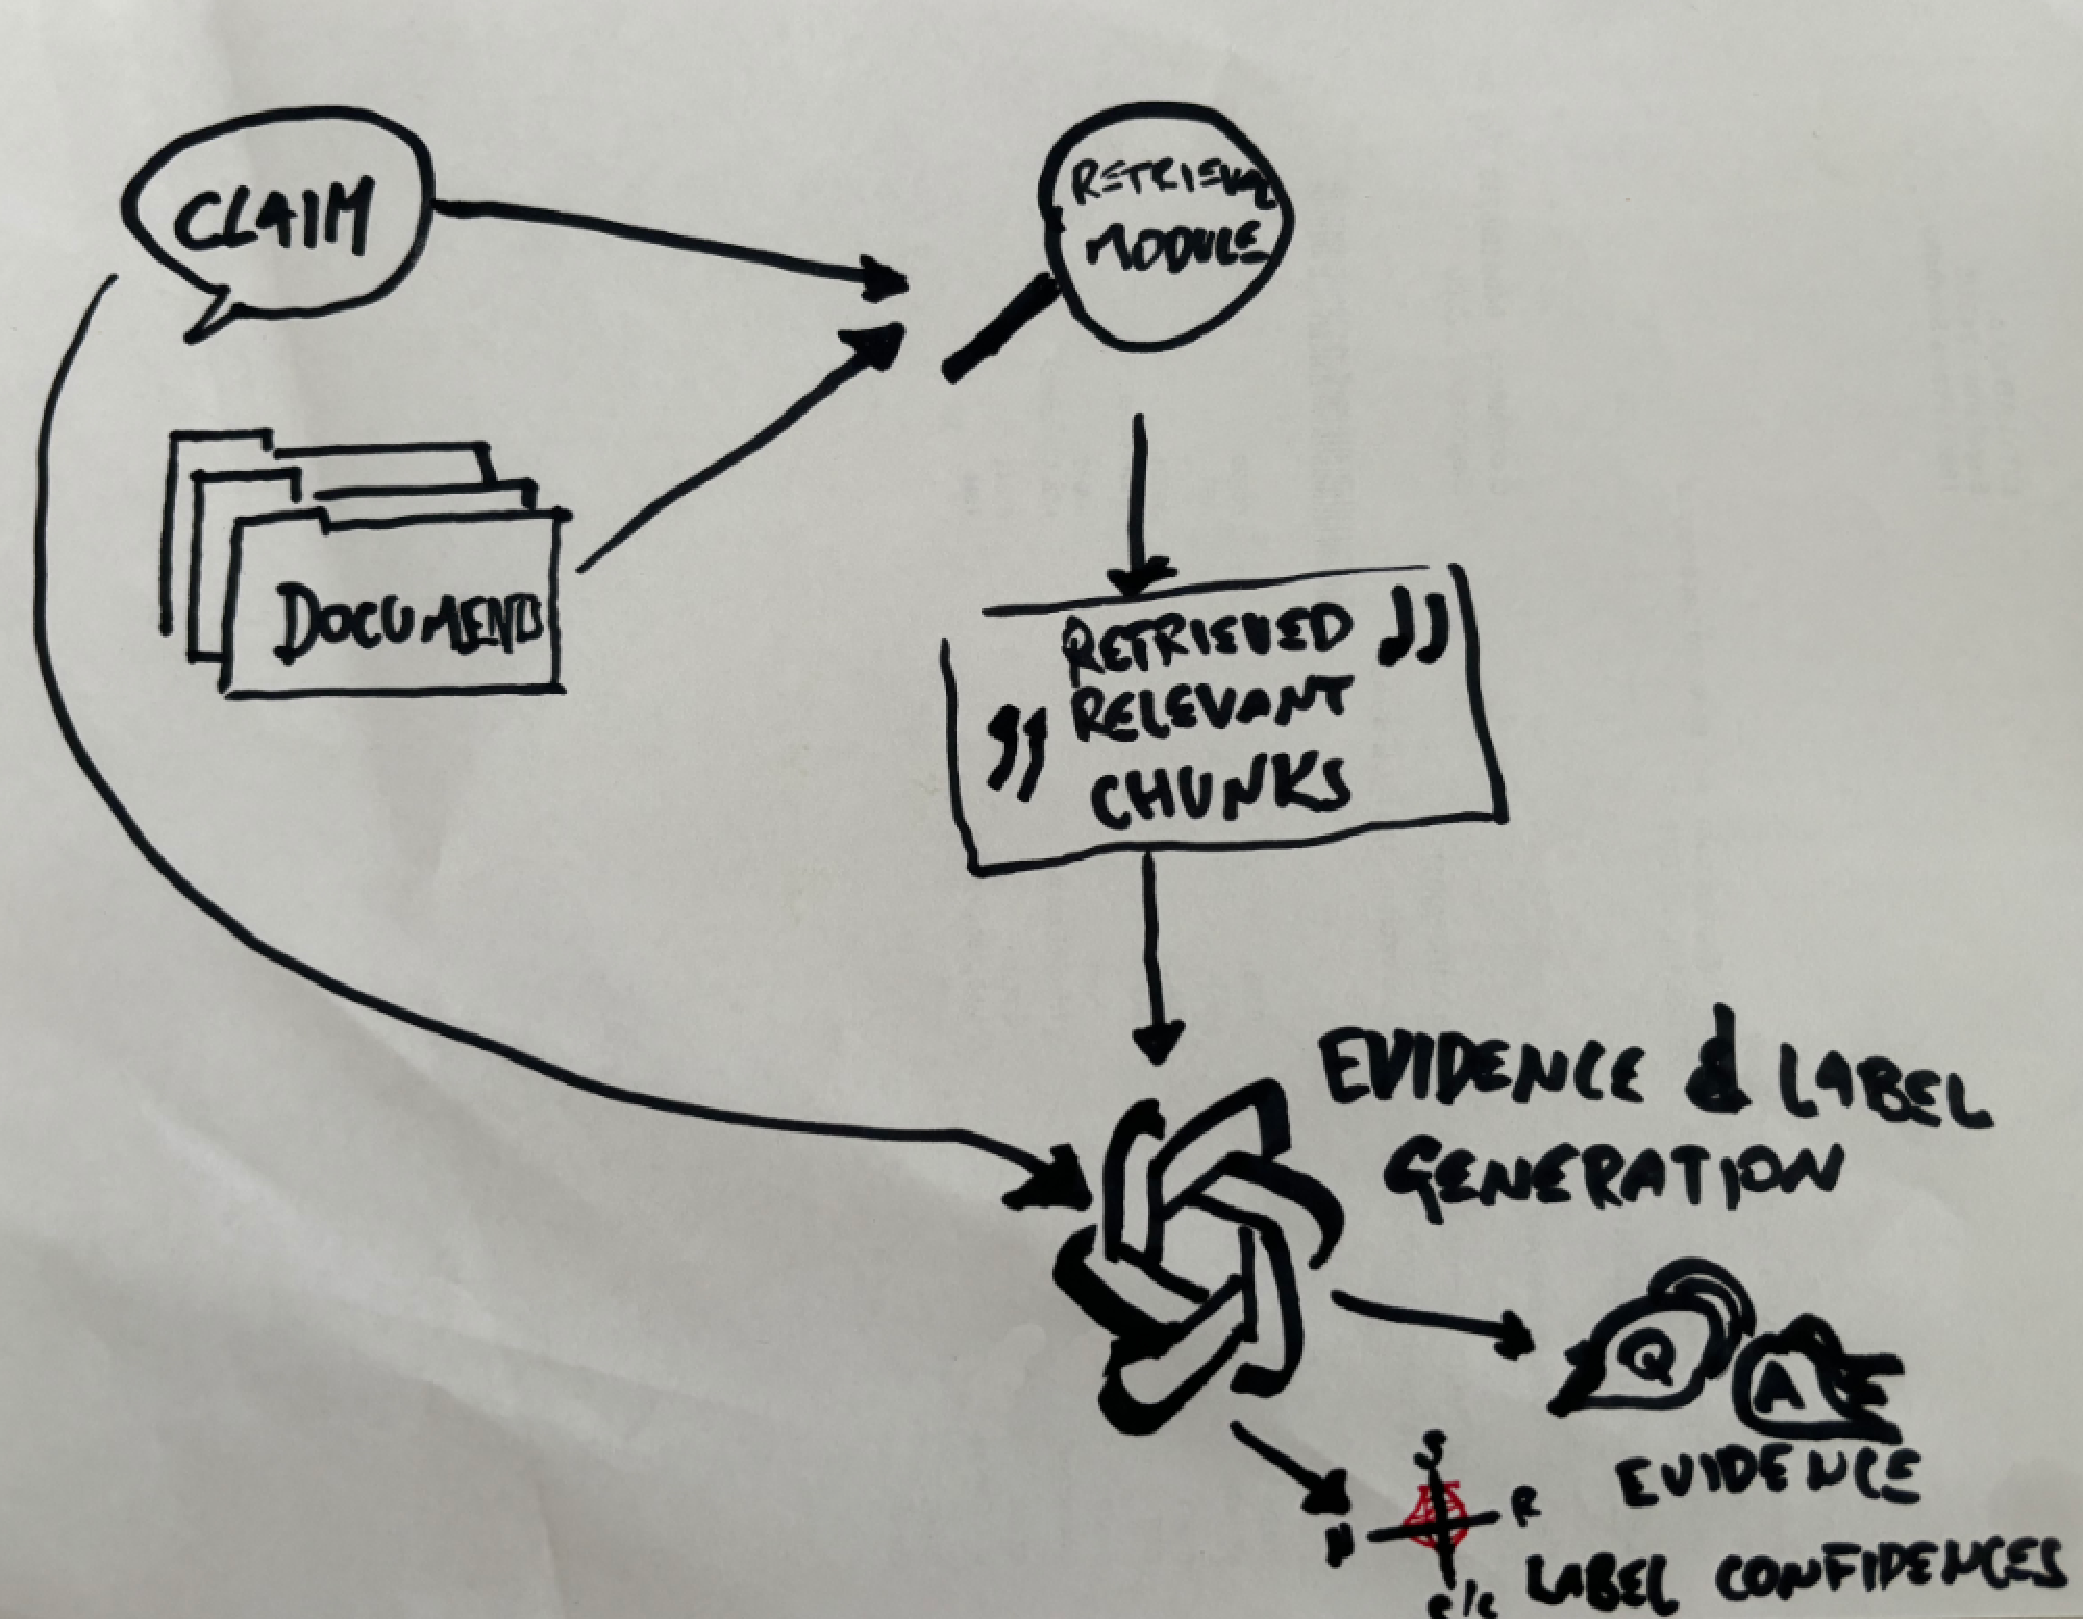
\includegraphics[width=0.47\textwidth]{figures/pipeline.pdf}
    \caption{Our pipeline}
    \label{fig:pipeline}
\end{figure}

\section{Related Work}
\label{sec:relwork}
\begin{enumerate}
    \item \textbf{\averitec{} score}~\cite{averitec2024} postulates method of unsupervised scoring of fact-checking pipeline against gold evidence and labels using Hungarian Meteor score and an accuracy metric
    \item \textbf{Baseline \averitec{} system} solves the task through 
    \item Our previous research on fact-checking pipelines~\cite{Ullrich2023,drchal2023pipelinedatasetgenerationautomated} using data similar to FEVER and \averitec{} shows significant superiority of fact-checking pipelines that \textbf{retrieve the whole documents} for the inference step, rather than out-of-context sentences
    \item \textbf{FEVER Shared Task}~\cite{thorne-etal-2018-fact} solutions such as Papelo~\cite{}
    \item \textbf{Retrieval-Augmented Generation (RAG) for Knowledge-Intensive Tasks}~\cite{rag} have demonstrated even simpler pipeline on the original FEVER dataset, 
\end{enumerate}

